\documentclass{ximera}

%\addPrintStyle{..}

\begin{document}
	\author{Bart Lambregs}
	\xmtitle{Gravitationele potentiële energie}{}
    \xmsource\xmuitleg


	\subsection{Gravitationele potentiële energie}

	Beschouw een massa op een hoogte boven het aardoppervlak. Vanuit deze positie kan ze arbeid verrichten en zal ze dus potentiële energie bezitten. Als we de massa bijvoorbeeld laten vallen kan ze op de grond een nagel inslaan en dus arbeid verrichten.
	
	\begin{image}
	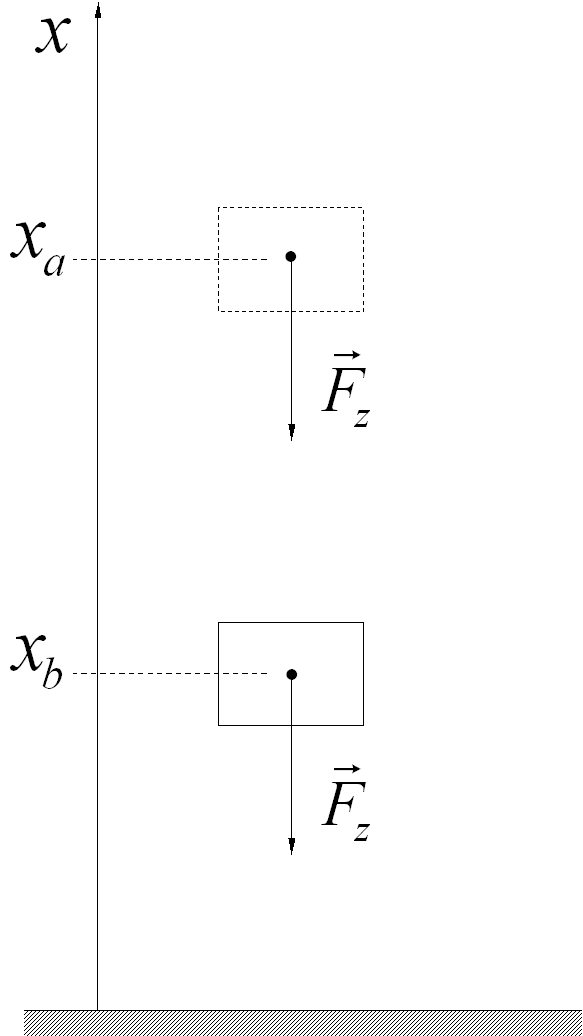
\includegraphics[height=5.5cm ,angle=0]{gravitationele_energie}
	\end{image}

	Bij het vallen van een hoogte $x_a$ naar een hoogte $x_b$ levert de zwaartekracht die aan de massa trekt een arbeid gelijk aan:
	\begin{eqnarray*}
	W\,=\,\int_{x_a}^{x_b}F_zdx\,=\,\int_{x_a}^{x_b}(-mg)dx\,=\,mgx_a-mgx_b
	\end{eqnarray*}
	Hier voldoet de uitdrukking $mgx$ aan wat we verwachten van potentiële ener\-gie. Het verschil van de uitdrukking geëvalueerd in het beginpunt en het eindpunt -- het verschil in energie -- is gelijk aan de hoeveelheid arbeid die tussen deze twee posities kan worden geleverd. We noemen de uitdrukking de \textit{gravitationele potentiële energie}. En als we $x$ door $h$ vervangen, krijgen we de gekende vorm:
	\begin{eqnarray}
	E_p&=&mgh
	\end{eqnarray}
	Net zoals bij de veerkracht geldt $W=-\Delta E_p$. 
	
	Waarom nu eigenlijk dat minteken? Als de massa valt, wordt door de zwaartekracht positieve arbeid verricht. Op een punt iets lager dan waar de massa was vertrokken, kan de massa nog minder ver vallen zodat ze vanuit dit punt minder arbeid kan leveren. Haar potentiële energie is afgenomen of de verandering $\Delta E_p$ is negatief. Dat wat aan potentiële energie verloren is gegaan, is aan arbeid geleverd. Als de massa omhoog wordt gegooid, heeft ze in een punt hoger dan daar waar ze vertrok meer potentiële energie. Vanaf een grotere hoogte kan ze meer arbeid leveren. De potentiële energie neemt dus toe of de verandering $\Delta E_p$ is positief. De zwaartekracht $F_z$ is echter tegengesteld (naar beneden gericht) aan de verplaatsing (naar boven) zodat de geleverde arbeid negatief is. Het toenemen van de energie kan maar mogelijk zijn als van elders energie aan de massa wordt gegeven. In dit geval is ze afkomstig van de kinetische energie die bij het opwerpen wordt meegegeven.
	
	Merk op dat de massa in staat is arbeid te verrichten als gevolg van het feit dat de zwaartekracht erop inwerkt en de massa bijgevolg \textit{zelf} een even grote kracht kan uitoefenen. Op die manier kunnen we de potentiële energie toekennen aan de massa; \textit{de massa} gaat op deze manier in staat zijn arbeid te verrichten.
	
\end{document}
